% Options for packages loaded elsewhere
\PassOptionsToPackage{unicode}{hyperref}
\PassOptionsToPackage{hyphens}{url}
%
\documentclass[
  man,floatsintext]{apa7}
\usepackage{amsmath,amssymb}
\usepackage{iftex}
\ifPDFTeX
  \usepackage[T1]{fontenc}
  \usepackage[utf8]{inputenc}
  \usepackage{textcomp} % provide euro and other symbols
\else % if luatex or xetex
  \usepackage{unicode-math} % this also loads fontspec
  \defaultfontfeatures{Scale=MatchLowercase}
  \defaultfontfeatures[\rmfamily]{Ligatures=TeX,Scale=1}
\fi
\usepackage{lmodern}
\ifPDFTeX\else
  % xetex/luatex font selection
\fi
% Use upquote if available, for straight quotes in verbatim environments
\IfFileExists{upquote.sty}{\usepackage{upquote}}{}
\IfFileExists{microtype.sty}{% use microtype if available
  \usepackage[]{microtype}
  \UseMicrotypeSet[protrusion]{basicmath} % disable protrusion for tt fonts
}{}
\makeatletter
\@ifundefined{KOMAClassName}{% if non-KOMA class
  \IfFileExists{parskip.sty}{%
    \usepackage{parskip}
  }{% else
    \setlength{\parindent}{0pt}
    \setlength{\parskip}{6pt plus 2pt minus 1pt}}
}{% if KOMA class
  \KOMAoptions{parskip=half}}
\makeatother
\usepackage{xcolor}
\usepackage{graphicx}
\makeatletter
\def\maxwidth{\ifdim\Gin@nat@width>\linewidth\linewidth\else\Gin@nat@width\fi}
\def\maxheight{\ifdim\Gin@nat@height>\textheight\textheight\else\Gin@nat@height\fi}
\makeatother
% Scale images if necessary, so that they will not overflow the page
% margins by default, and it is still possible to overwrite the defaults
% using explicit options in \includegraphics[width, height, ...]{}
\setkeys{Gin}{width=\maxwidth,height=\maxheight,keepaspectratio}
% Set default figure placement to htbp
\makeatletter
\def\fps@figure{htbp}
\makeatother
\setlength{\emergencystretch}{3em} % prevent overfull lines
\providecommand{\tightlist}{%
  \setlength{\itemsep}{0pt}\setlength{\parskip}{0pt}}
\setcounter{secnumdepth}{-\maxdimen} % remove section numbering
% Make \paragraph and \subparagraph free-standing
\ifx\paragraph\undefined\else
  \let\oldparagraph\paragraph
  \renewcommand{\paragraph}[1]{\oldparagraph{#1}\mbox{}}
\fi
\ifx\subparagraph\undefined\else
  \let\oldsubparagraph\subparagraph
  \renewcommand{\subparagraph}[1]{\oldsubparagraph{#1}\mbox{}}
\fi
\newlength{\cslhangindent}
\setlength{\cslhangindent}{1.5em}
\newlength{\csllabelwidth}
\setlength{\csllabelwidth}{3em}
\newlength{\cslentryspacingunit} % times entry-spacing
\setlength{\cslentryspacingunit}{\parskip}
\newenvironment{CSLReferences}[2] % #1 hanging-ident, #2 entry spacing
 {% don't indent paragraphs
  \setlength{\parindent}{0pt}
  % turn on hanging indent if param 1 is 1
  \ifodd #1
  \let\oldpar\par
  \def\par{\hangindent=\cslhangindent\oldpar}
  \fi
  % set entry spacing
  \setlength{\parskip}{#2\cslentryspacingunit}
 }%
 {}
\usepackage{calc}
\newcommand{\CSLBlock}[1]{#1\hfill\break}
\newcommand{\CSLLeftMargin}[1]{\parbox[t]{\csllabelwidth}{#1}}
\newcommand{\CSLRightInline}[1]{\parbox[t]{\linewidth - \csllabelwidth}{#1}\break}
\newcommand{\CSLIndent}[1]{\hspace{\cslhangindent}#1}
\ifLuaTeX
\usepackage[bidi=basic]{babel}
\else
\usepackage[bidi=default]{babel}
\fi
\babelprovide[main,import]{english}
% get rid of language-specific shorthands (see #6817):
\let\LanguageShortHands\languageshorthands
\def\languageshorthands#1{}
% Manuscript styling
\usepackage{upgreek}
\captionsetup{font=singlespacing,justification=justified}

% Table formatting
\usepackage{longtable}
\usepackage{lscape}
% \usepackage[counterclockwise]{rotating}   % Landscape page setup for large tables
\usepackage{multirow}		% Table styling
\usepackage{tabularx}		% Control Column width
\usepackage[flushleft]{threeparttable}	% Allows for three part tables with a specified notes section
\usepackage{threeparttablex}            % Lets threeparttable work with longtable

% Create new environments so endfloat can handle them
% \newenvironment{ltable}
%   {\begin{landscape}\centering\begin{threeparttable}}
%   {\end{threeparttable}\end{landscape}}
\newenvironment{lltable}{\begin{landscape}\centering\begin{ThreePartTable}}{\end{ThreePartTable}\end{landscape}}

% Enables adjusting longtable caption width to table width
% Solution found at http://golatex.de/longtable-mit-caption-so-breit-wie-die-tabelle-t15767.html
\makeatletter
\newcommand\LastLTentrywidth{1em}
\newlength\longtablewidth
\setlength{\longtablewidth}{1in}
\newcommand{\getlongtablewidth}{\begingroup \ifcsname LT@\roman{LT@tables}\endcsname \global\longtablewidth=0pt \renewcommand{\LT@entry}[2]{\global\advance\longtablewidth by ##2\relax\gdef\LastLTentrywidth{##2}}\@nameuse{LT@\roman{LT@tables}} \fi \endgroup}

% \setlength{\parindent}{0.5in}
% \setlength{\parskip}{0pt plus 0pt minus 0pt}

% Overwrite redefinition of paragraph and subparagraph by the default LaTeX template
% See https://github.com/crsh/papaja/issues/292
\makeatletter
\renewcommand{\paragraph}{\@startsection{paragraph}{4}{\parindent}%
  {0\baselineskip \@plus 0.2ex \@minus 0.2ex}%
  {-1em}%
  {\normalfont\normalsize\bfseries\itshape\typesectitle}}

\renewcommand{\subparagraph}[1]{\@startsection{subparagraph}{5}{1em}%
  {0\baselineskip \@plus 0.2ex \@minus 0.2ex}%
  {-\z@\relax}%
  {\normalfont\normalsize\itshape\hspace{\parindent}{#1}\textit{\addperi}}{\relax}}
\makeatother

\makeatletter
\usepackage{etoolbox}
\patchcmd{\maketitle}
  {\section{\normalfont\normalsize\abstractname}}
  {\section*{\normalfont\normalsize\abstractname}}
  {}{\typeout{Failed to patch abstract.}}
\patchcmd{\maketitle}
  {\section{\protect\normalfont{\@title}}}
  {\section*{\protect\normalfont{\@title}}}
  {}{\typeout{Failed to patch title.}}
\makeatother

\usepackage{xpatch}
\makeatletter
\xapptocmd\appendix
  {\xapptocmd\section
    {\addcontentsline{toc}{section}{\appendixname\ifoneappendix\else~\theappendix\fi\\: #1}}
    {}{\InnerPatchFailed}%
  }
{}{\PatchFailed}
\usepackage{lineno}

\linenumbers
\usepackage{csquotes}
\usepackage{amsmath}
\usepackage{amssymb}
\usepackage{unicode-math}
\usepackage{setspace}
\usepackage{libertine}
\captionsetup[figure]{font={stretch=1}}
\makeatletter
\renewcommand{\paragraph}{\@startsection{paragraph}{4}{\parindent}%
  {0\baselineskip \@plus 0.2ex \@minus 0.2ex}%
  {-1em}%
  {\normalfont\normalsize\bfseries\typesectitle}}

\renewcommand{\subparagraph}[1]{\@startsection{subparagraph}{5}{1em}%
  {0\baselineskip \@plus 0.2ex \@minus 0.2ex}%
  {-\z@\relax}%
  {\normalfont\normalsize\bfseries\itshape\hspace{\parindent}{#1}\textit{\addperi}}{\relax}}
\makeatother
\ifLuaTeX
  \usepackage{selnolig}  % disable illegal ligatures
\fi
\IfFileExists{bookmark.sty}{\usepackage{bookmark}}{\usepackage{hyperref}}
\IfFileExists{xurl.sty}{\usepackage{xurl}}{} % add URL line breaks if available
\urlstyle{same}
\hypersetup{
  pdftitle={A universal of human social cognition: Children from 17 communities process gaze in similar ways},
  pdfauthor={Manuel Bohn1,2,*, Julia Christin Prein1,2,*, Agnes Ayikoru3, Florian M. Bednarski4, Ardain Dzabatou5, Michael C. Frank6, Annette M. E. Henderson4, Joan Isabella3, Josefine Kalbitz2, Patricia Kanngiesser7, Dilara Keşşafoğlu8, Bahar Köymen9, Maira V. Manrique-Hernandez2, Shirley Magazi10, Lizbeth Mújica-Manrique2, Julia Ohlendorf2, Damilola Olaoba2, Wesley R. Pieters10, Sarah Pope-Caldwell2, Katie Slocombe11, Robert Z. Sparks6, Jahnavi Sunderarajan2, Wilson Vieira2, Zhen Zhang12, Yufei Zong12, Roman Stengelin2,10,+, \& Daniel B. M. Haun2,+},
  pdflang={en-EN},
  hidelinks,
  pdfcreator={LaTeX via pandoc}}

\title{A universal of human social cognition: Children from 17 communities process gaze in similar ways}
\author{Manuel Bohn\textsuperscript{1,2,*}, Julia Christin Prein\textsuperscript{1,2,*}, Agnes Ayikoru\textsuperscript{3}, Florian M. Bednarski\textsuperscript{4}, Ardain Dzabatou\textsuperscript{5}, Michael C. Frank\textsuperscript{6}, Annette M. E. Henderson\textsuperscript{4}, Joan Isabella\textsuperscript{3}, Josefine Kalbitz\textsuperscript{2}, Patricia Kanngiesser\textsuperscript{7}, Dilara Keşşafoğlu\textsuperscript{8}, Bahar Köymen\textsuperscript{9}, Maira V. Manrique-Hernandez\textsuperscript{2}, Shirley Magazi\textsuperscript{10}, Lizbeth Mújica-Manrique\textsuperscript{2}, Julia Ohlendorf\textsuperscript{2}, Damilola Olaoba\textsuperscript{2}, Wesley R. Pieters\textsuperscript{10}, Sarah Pope-Caldwell\textsuperscript{2}, Katie Slocombe\textsuperscript{11}, Robert Z. Sparks\textsuperscript{6}, Jahnavi Sunderarajan\textsuperscript{2}, Wilson Vieira\textsuperscript{2}, Zhen Zhang\textsuperscript{12}, Yufei Zong\textsuperscript{12}, Roman Stengelin\textsuperscript{2,10,+}, \& Daniel B. M. Haun\textsuperscript{2,+}}
\date{}


\shorttitle{gaze following across 17 communities}

\authornote{

The authors would like to thank Luke Maurits for statistical advice. Manuel Bohn was supported by a Jacobs Foundation Research Fellowship (2022-1484-00). We are grateful to thank all children and caregivers for participating in the study. We thank the Max Planck Society for the Advancement of Science.

The authors made the following contributions. Manuel Bohn: Conceptualization, Methodology, Formal Analysis, Writing - Original Draft Preparation, Writing - Review \& Editing; Julia Christin Prein: Conceptualization, Methodology, Software, Investigation, Writing - Review \& Editing; Agnes Ayikoru: Investigation; Florian M. Bednarski: Investigation, Writing - Review \& Editing; Ardain Dzabatou: Investigation; Michael C. Frank: Investigation, Writing - Review \& Editing; Annette M. E. Henderson: Investigation, Writing - Review \& Editing; Joan Isabella: Investigation; Josefine Kalbitz: Investigation, Writing - Review \& Editing; Patricia Kanngiesser: Investigation, Writing - Review \& Editing; Dilara Keşşafoğlu: Investigation, Writing - Review \& Editing; Bahar Köymen: Investigation, Writing - Review \& Editing; Maira V. Manrique-Hernandez: Investigation; Shirley Magazi: Investigation; Lizbeth Mújica-Manrique: Investigation, Writing - Review \& Editing; Julia Ohlendorf: Investigation; Damilola Olaoba: Investigation; Wesley R. Pieters: Investigation, Writing - Review \& Editing; Sarah Pope-Caldwell: Investigation; Katie Slocombe: Investigation, Writing - Review \& Editing; Robert Z. Sparks: Investigation; Jahnavi Sunderarajan: Investigation; Wilson Vieira: Investigation; Zhen Zhang: Investigation, Writing - Review \& Editing; Yufei Zong: Investigation; Roman Stengelin: Conceptualization, Methodology, Investigation, Writing - Review \& Editing; Daniel B. M. Haun: Conceptualization, Funding acquisition, Writing - Review \& Editing.

Correspondence concerning this article should be addressed to Manuel Bohn, Universitätsallee 1, 21335 Lüneburg, Germany. E-mail: \href{mailto:manuel.bohn@leuphana.de}{\nolinkurl{manuel.bohn@leuphana.de}}

}

\affiliation{\vspace{0.5cm}\textsuperscript{1} Institute of Psychology in Education, Leuphana University Lüneburg\\\textsuperscript{2} Department of Comparative Cultural Psychology, Max Planck Institute for Evolutionary Anthropology\\\textsuperscript{3} Budongo Conservation Field Station\\\textsuperscript{4} School of Psychology, University of Auckland\\\textsuperscript{5} Université Marien Ngouabi\\\textsuperscript{6} Department of Psychology, Stanford University\\\textsuperscript{7} School of Psychology, University of Plymouth\\\textsuperscript{8} Department of Psychology, Koç University\\\textsuperscript{9} Division of Psychology, Communication, and Human Neuroscience, University of Manchester\\\textsuperscript{10} Department of Psychology and Social Work, University of Namibia\\\textsuperscript{11} Department of Psychology, University of York\\\textsuperscript{12} CAS Key Laboratory of Behavioral Science, Institute of Psychology, Chinese Academy of Sciences\\\textsuperscript{*} joint first author\\\textsuperscript{+} joint last author}

\abstract{%
Theoretical accounts assume that key features of human social cognition are universal. Here we focus on gaze following, the bedrock of social interactions and coordinated activities, to test this claim. In a comprehensive cross-cultural study spanning five continents and 17 distinct cultural communities, we examined the development of gaze following in early childhood. We identified key processing signatures through a computational model that assumes that participants follow an individual's gaze by estimating a vector emanating from the eye center through the pupil. We found these signatures in all communities, suggesting that children worldwide processed gaze in highly similar ways. Absolute differences between groups were accounted for by a cross-culturally consistent relationship between children's exposure to touchscreens and their performance in the task. These results provide strong evidence for a universal process underlying a foundational socio-cognitive ability in humans that can be reliably inferred even in the presence of cultural variation in overt behavior.
}



\begin{document}
\maketitle

\hypertarget{introduction}{%
\section{Introduction}\label{introduction}}

Human socio-cognitive skills enable unique forms of communication and cooperation that provide a bedrock for cumulative culture and the formation of complex societies (Henrich, 2016; Heyes, 2018; Laland \& Seed, 2021; Legare, 2019; Tomasello, 2020; Tomasello \& Rakoczy, 2003; Wellman, 2014). The eyes are the proverbial ``window to the mind'' and eye gaze is essential for many social reasoning processes (Doherty, 2006; Emery, 2000; Frischen et al., 2007; Shepherd, 2010). Others' eye gaze is used to infer their focus of visual attention, which is a critical aspect of coordinated activities, including communication and cooperation (Langton et al., 2000; Richardson \& Dale, 2005; Rossano, 2012; Scaife \& Bruner, 1975; Sebanz et al., 2006; Tomasello et al., 2007). During ontogeny, gaze following is an important aspect of many critical learning objectives that enable children to become functioning members of the society they grow up in, including language, social learning and joint action (Brooks \& Meltzoff, 2005; Brownell, 2011; Carpenter et al., 1998; Moore, 2008; Mundy \& Newell, 2007; Stephenson et al., 2021). Because of the central role gaze following plays during human ontogeny, it has been widely argued that gaze following has been a target of natural selection (Clark et al., 2023; Emery, 2000; Kano, 2023; Tomasello et al., 2007). This implies that the process by which humans use gaze direction to infer the focus of attention is universal. In this paper, we report a comprehensive cross-cultural study on the ontogeny of gaze following in which we shed light on the universal aspects of gaze following as well as sources of variation and their origins.

\hypertarget{ontogeny-of-gaze-following}{%
\subsection{Ontogeny of gaze following}\label{ontogeny-of-gaze-following}}

The ability to follow gaze emerges early in development (Byers-Heinlein et al., 2021; Del Bianco et al., 2019; Gredebäck et al., 2010; Tang et al., 2023). The earliest signs of gaze following have been found in infants as young as four months (Astor et al., 2021; D'Entremont et al., 1997). Throughout the first two years of life, children refine their abilities: they interpret gaze in mentalistic terms (Butterworth \& Jarrett, 1991; Deák et al., 2000), for example, they follow gaze to locations outside their own visual field by moving around barriers (Moll \& Tomasello, 2004). Initially, children rely more on head direction than actual gaze direction (Michel et al., 2021). In fact, when head and gaze direction diverge, children fail to accurately locate the agent's focus of attention up until 19 months of age (Lempers, 1979).

From an evolutionary perspective, while many species are able to follow gaze based on head directions, uniquely human forms of joint action and communication require a more precise localization of other's attention and thus critically rely on gaze direction inferred from eye movements (Emery, 2000; Hessels, 2020). In a recent study, Prein, Maurits, et al. (2024) studied the development of gaze following based on eye movements across from three years up until old age. They found particularly steep developmental improvements in the preschool years resulting in a relatively stable level of accuracy from ten years onward and a slight decrease starting around age 40.

The studies reported thus far, all relied on data collected in western affluent settings. Such settings represent only a minority of the worlds population and are thus insufficient to make claims about universal aspects of human cognition (Amir \& McAuliffe, 2020; Nielsen et al., 2017; Norenzayan \& Heine, 2005). Three studies with infants and children from traditionally underrepresented parts of the world (Bhutan, India, Peru, Vanuatu) find that children start gaze following (including head direction) at similar ages, the rates of gaze following, however, differed between cultural settings (Astor et al., 2022; Callaghan et al., 2011; Hernik \& Broesch, 2019).

Rates and accuracy of gaze following do not just differ between cultural settings; there is also substantial variation within settings. In fact, the pivotal role of gaze following in many uniquely human activities has been studied by relating individual differences in gaze following to other phenomena -- both cross-sectionally and longitudinally (Brooks \& Meltzoff, 2015; Carpenter et al., 1998). For example, gaze following at 10 months predicts language scores at 18 months of age (Brooks \& Meltzoff, 2005; see also Macdonald \& Tatler, 2013). Furthermore, difficulties with gaze following have been linked to developmental disorders, including Autism (Itier \& Batty, 2009; Thorup et al., 2016, 2018) and -- at least in some cultural contexts -- to maternal postpartum depression {[}astor2022maternal{]}. Individual differences are also key to explaining the -- mainly social-interactional -- driving forces behind the development of gaze following. For example, it has been found that early attachment quality or the use of gaze in communicative interactions predict later rates of gaze following (Astor et al., 2020; Movellan \& Watson, 2002; Senju et al., 2015).

\hypertarget{cognitive-universals-and-sources-of-variation}{%
\subsection{Cognitive universals and sources of variation}\label{cognitive-universals-and-sources-of-variation}}

The existence of variation in gaze following both within and between cultural settings raises the question of how to square these findings with the suggestion that gaze following is a fundamental building block of human social cognition and interaction and that eye movements are processed the same way in humans all over the world. Looking at other aspects of social cognition, one could easily make the argument that variation is the norm rather than the exception (Dixson et al., 2018; Mayer \& Träuble, 2013; see e.g., Miller et al., 2018; Taumoepeau et al., 2019; Wellman, 2014). As a first step, answering this question requires data from many different cultural settings. In a second step, however, we need to a way of detecting universal processes in such data. The traditional approach is to compare some sort of aggregate measure (mean level of performance, average age of onset) across cultural settings. Absolute differences in mean performance across communities are interpreted as a signal of different underlying cognitive processes (Blake et al., 2015; see e.g., House et al., 2020; Kanngiesser et al., 2022; Van Leeuwen et al., 2018). No differences seemingly support the existence of a psychological universal. Such an approach, however, neglects the existence of within-cultural variation altogether (see also Gurven, 2018).

In the present study, we want to take a different approach for which we assume that universal processes and variation can co-exist (Greenfield et al., 2003; Jensen, 2012; Kline et al., 2018). Instead of starting with the outcome (performance in the task), we start with the process that generates the outcome. By defining this process, we make a proposal for the universal aspect of the process. At the same time, we define variable aspects in the process that generate individual differences. This allows us to define signatures that the process leaves behind that can be detected independent of absolute levels of performance.

For gaze following, we can use the computational model proposed by Prein, Maurits, et al. (2024) to derive such predictions. They formalized the widely-held view that gaze following involves estimating a vector emanating from the eye center through the pupil (Butterworth \& Jarrett, 1991; Symons et al., 2004; Todorović, 2006; Yaniv \& Shatz, 1990). The key innovation of the model is that it explains how individuals may use the same process but still differ in their measured abilities. The process always involves estimating a vector but also involves a degree of uncertainty because the eye center is not directly observable. Individuals are assumed to differ in their level of uncertainty with which they estimate the vector which causes differences in their observable behavior. Importantly, the assumed process leaves a key signature in the data that is observable independent of the absolute level of performance. In the present study, we therefore focus on this signature instead of absolute levels of performance when evaluating the claim whether there is evidence for a universal cognitive process underlying gaze following.

\hypertarget{the-current-study}{%
\subsection{The current study}\label{the-current-study}}

The present study had three goals. First, to collect a comprehensive data set and study the ontogeny of gaze following beyond infancy across cultures. To make this possible, we used a semi-standardized task that required minimal assistance from an experimenter and no behavioral coding. The task is an animated picture book presented on a tablet screen. Children watched a balloon disappear behind a hedge. An agent followed the trajectory of the balloon with their eyes (Figure \ref{fig:fig1}B). The key dependent variable was (im)precision, that is, the deviation between where the agent looked (where the balloon was) and the child's response. The task's flexible implementation as a browser-based web-app allowed us to quickly tailor its visual and audio content to each cultural setting (visuals and audio). The task has been psychometrically evaluated and has shown to yield reliable individual-level measurements across communities and across ages (Prein, Kalinke, et al., 2024; Prein, Bednarski, et al., 2024).

We collected data in 17 different communities across 14 countries and five continents. Communities covered a broad spectrum of geographical locations, social and political systems, languages, and subsistence styles. This diversity allowed us to overcome a common pitfall of cross-cultural studies that compare urban communities from the Global North to rural communities from the Global South (Barrett, 2020). We aimed for large sample sizes within each community to contrast within- and between cultural variation. Our expectation regarding the first goal was to see substantial variation across cultures but even more variation between individuals. In all communities, we expected performance to increase with age.

The second goals was to look for signatures in the data of the universal gaze following process predicted by the model of Prein, Bednarski, et al. (2024). In the task, the hidden object is located on a horizontal plane at the lower end of the screen. The agent is located in the upper center of the screen (see Figure \ref{fig:fig1}B). The model predicts trials in which the object is hidden further away from the center to be more difficult resulting in higher imprecision. The signature is thus a u-shaped relation between object location and imprecision (Figure \ref{fig:fig12}).

Finally, we sought to explain individual differences in gaze following precision by linking them to methodological aspects of the study as well as aggregate measures of children's everyday social experience. Experience with tablets and touch screens co-varied with community and we expected children more familiar with this medium to perform better. Previous work suggested that gaze following is refined in social interaction (Movellan \& Watson, 2002; Senju et al., 2015). To approximate social interaction, we asked parents to fill out a questionnaire about household size and composition. We acknowledge that this measure approximates opportunities for social interaction in a rather crude way but we nevertheless expected children living in larger households and with more siblings (relative to their community) to be more accurate when following gaze.

\begin{figure}

{\centering 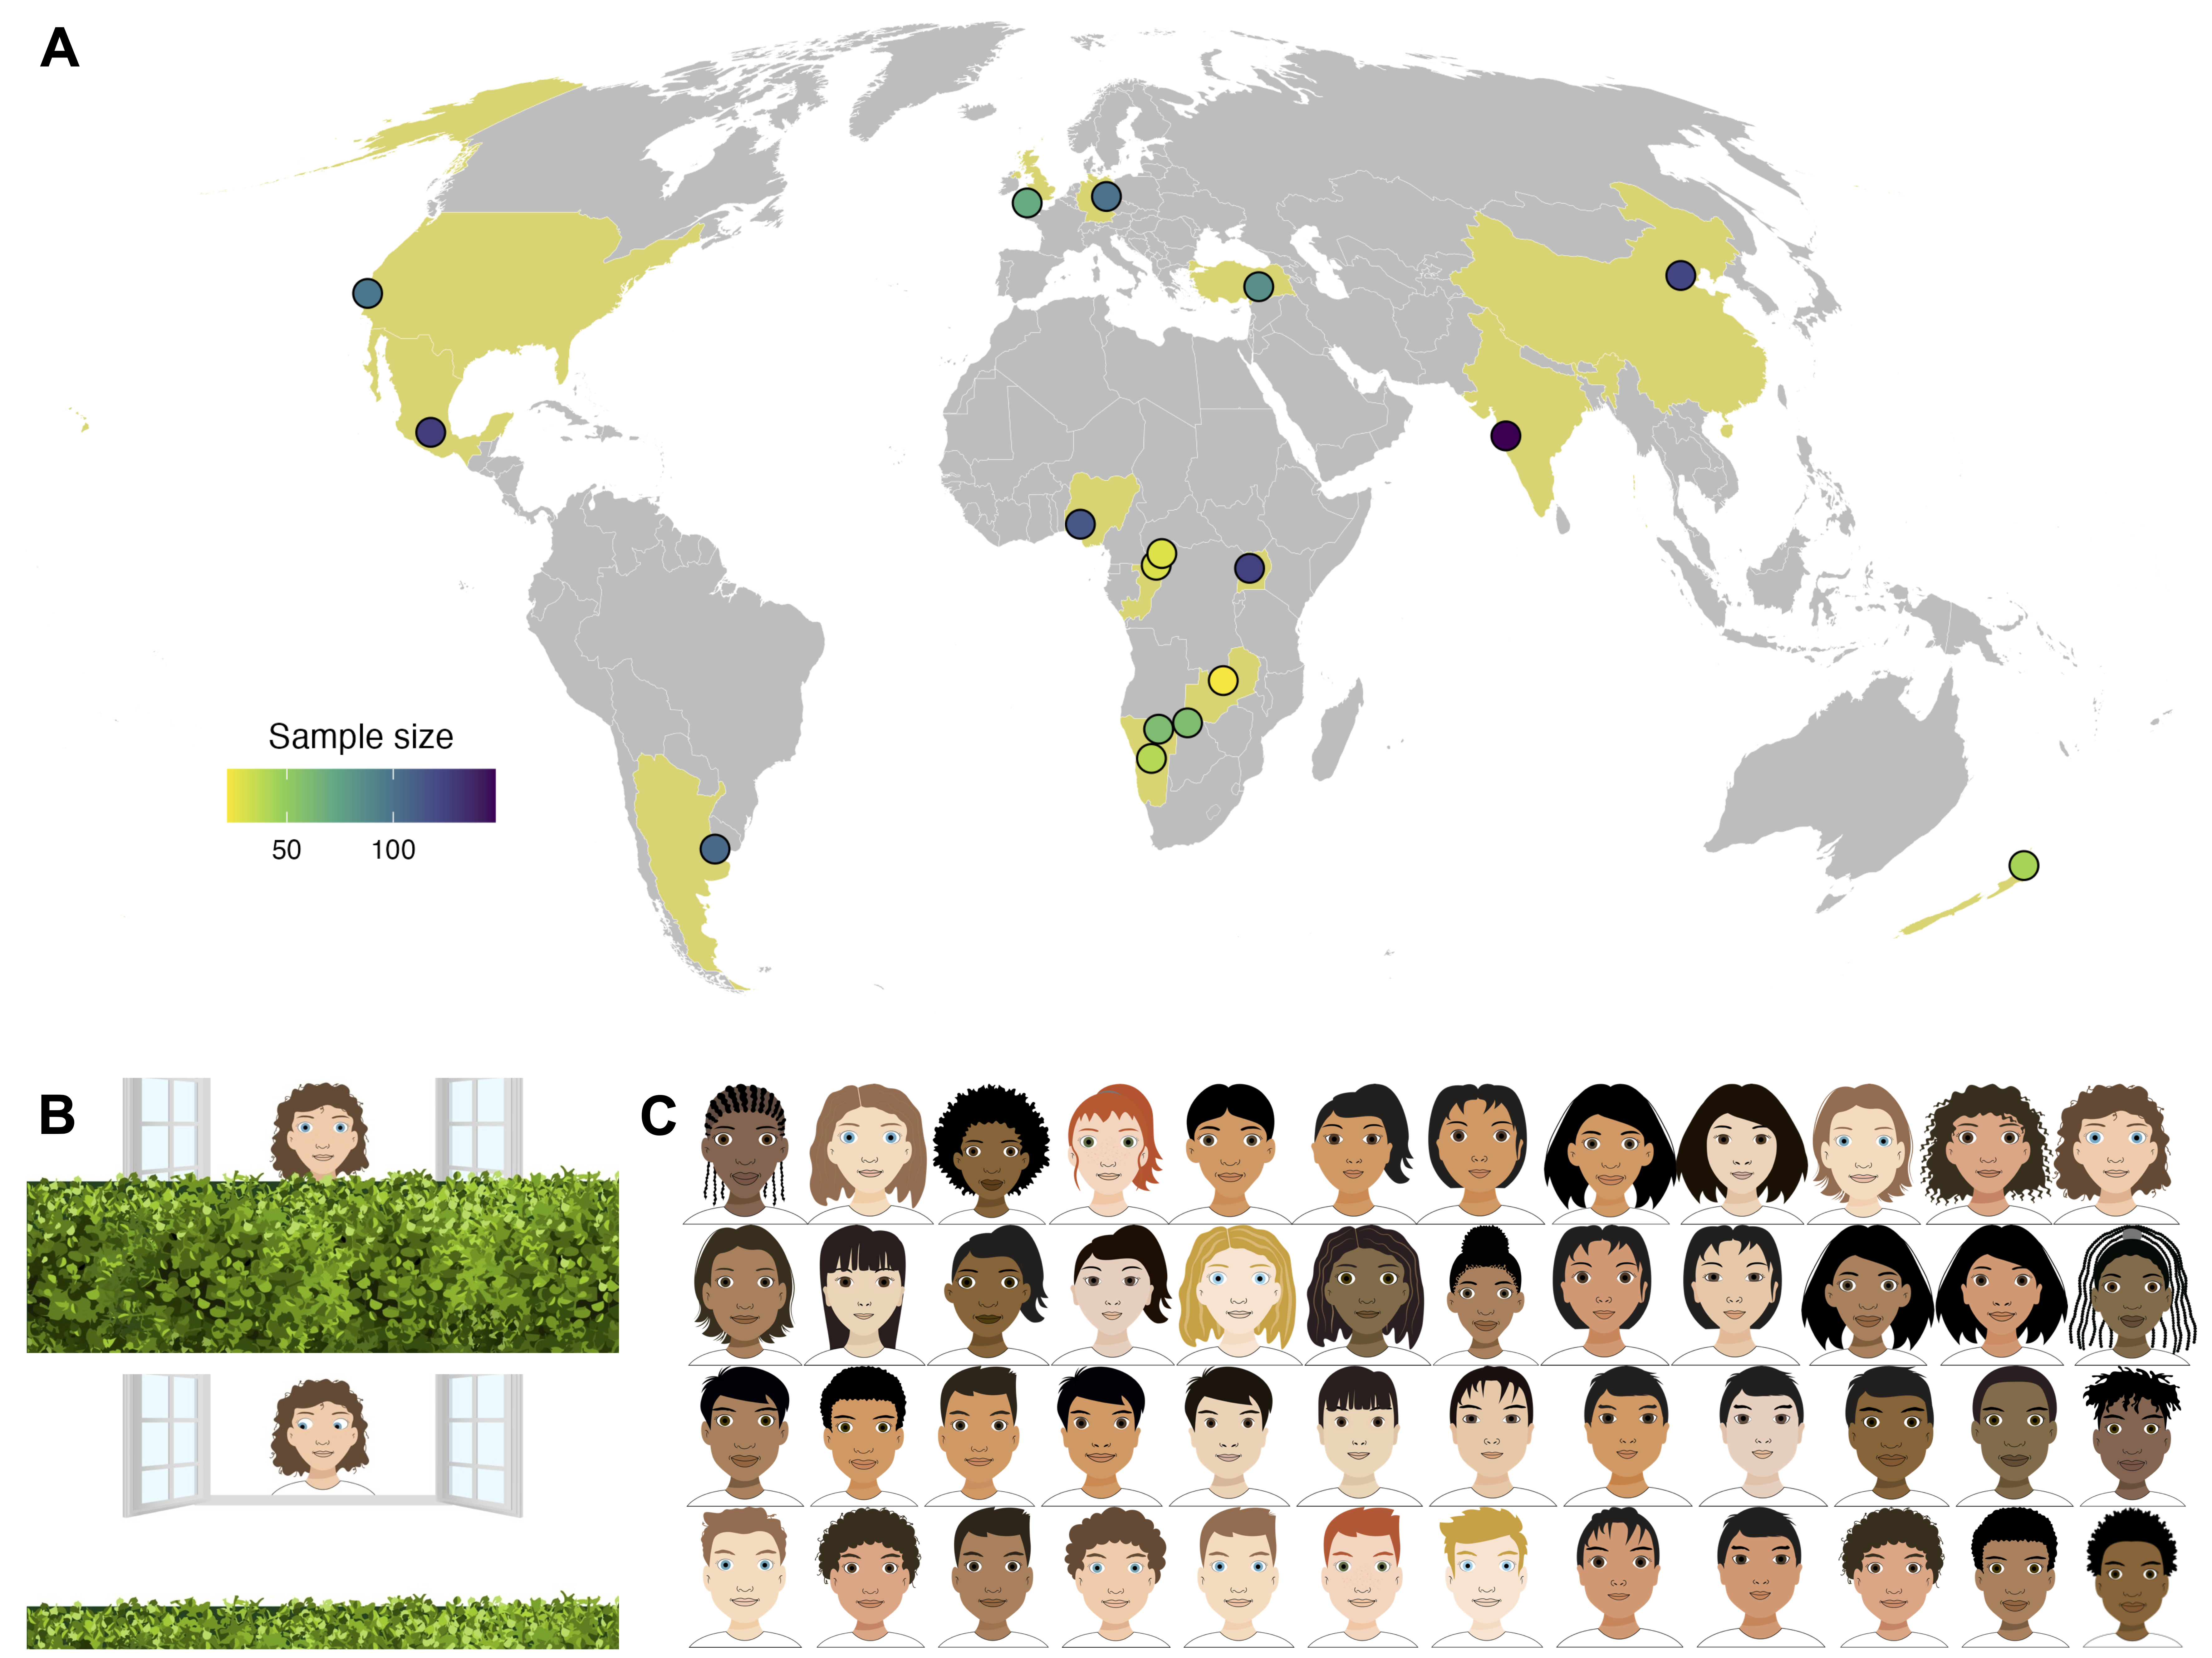
\includegraphics[width=1\linewidth]{../figures/fig1_2} 

}

\caption{(A) Data collection sites. Points show the approximate geographical location of the data collection sites, coloring shows the sample sizes. (B) Screenshots from the task. The upper scene depicts the start, and the lower scene depicts the choice phase in a test trial. Participants had to use the gaze of the agent to locate the balloon and touch the location on the hedge where they thought the balloon was. Agents, audio recordings and backgrounds were adapted to each community. (C) Drawings used as agents across communities.}\label{fig:fig1}
\end{figure}

\begin{center}
\begin{ThreePartTable}

\begin{TableNotes}[para]
\normalsize{\textit{Note.} 1 Proportion of participants who have access to touchscreens according to parental questionnaire. 2 Local collaborators and piloting suggested that Nigerian English is suitable for Windhoek as well.}
\end{TableNotes}

\begin{longtable}{m{0.125\linewidth}m{0.125\linewidth}m{0.125\linewidth}m{0.125\linewidth}m{0.125\linewidth}m{0.125\linewidth}m{0.125\linewidth}}\noalign{\getlongtablewidth\global\LTcapwidth=\longtablewidth}
\caption{\label{tab:tab1}Participant demographics.}\\
\toprule
Continent & Country & Community & N (male) & Age (range) & Language & Touchscreen exposure1\\
\midrule
\endfirsthead
\caption*{\normalfont{Table \ref{tab:tab1} continued}}\\
\toprule
Continent & Country & Community & N (male) & Age (range) & Language & Touchscreen exposure1\\
\midrule
\endhead
Americas & Argentina & Buenos Aires & 105 (53) & 4.72 (3.00 - 6.96) & Spanish (Rioplatense) & 0.90\\
 & México & Ocuilan & 127 (63) & 4.96 (2.57 - 6.95) & Spanish (Mexican) & 0.77\\
 & USA & Stanford & 98 (54) & 4.99 (2.52 - 7.90) & English (American) & 0.98\\
Africa & Namibia & Hai||om & 60 (38) & 5.85 (2.74 - 8.34) & Hai||om & 0.05\\
 &  & Khwe & 59 (24) & 5.84 (3.38 - 8.63) & Khwedam & 0.19\\
 &  & Windhoek & 39 (17) & 5.69 (2.66 - 8.66) & English (Nigerian)2 & 0.95\\
 & Nigeria & Akure & 114 (54) & 5.07 (2.57 - 7.33) & English (Nigerian) & 0.91\\
 & Rep. Congo & BaYaka & 29 (13) & 7.80 (3.94 - 10.56) & Yaka & 0.00\\
 &  & Bandongo & 30 (11) & 7.45 (3.50 - 10.95) & Lingala & 0.00\\
 & Uganda & Nyabyeya & 125 (62) & 5.94 (2.67 - 8.92) & Kiswahili & 0.34\\
 & Zambia & Chimfunshi & 22 (5) & 5.98 (2.88 - 8.00) & Bemba & 0.14\\
Europe & Germany & Leipzig & 100 (48) & 4.88 (2.53 - 6.95) & German & 0.89\\
 & UK & Plymouth & 70 (30) & 6.02 (2.38 - 8.94) & English (British) & 0.99\\
Asia & China & Beijing & 123 (62) & 5.47 (2.69 - 8.48) & Mandarin & 0.95\\
 & India & Pune & 148 (73) & 6.14 (3.06 - 8.83) & English (Indian) / Marathi & 0.93\\
 & Türkiye & Malatya & 85 (40) & 5.02 (2.75 - 7.12) & Turkish & 1.00\\
Oceania & New Zealand & Auckland & 43 (19) & 5.14 (2.81 - 8.75) & English (New Zealand) & 0.95\\
\bottomrule
\addlinespace
\insertTableNotes
\end{longtable}

\end{ThreePartTable}
\end{center}

We used an animated picture book tablet task in which participants had to locate a hidden object based on observing an agent's gaze. Children watched a balloon disappear behind a hedge. An agent followed the trajectory of the balloon with their eyes (Fig. \ref{fig:fig1}B). The key dependent variable was the (im)precision with which children located the agent's focus of attention, that is, the deviation between where the agent looked (where the balloon was) and the child's response. We adapted visuals and audio instructions specifically for each of the 17 communities. Previous work demonstrated excellent individual-level measurement properties for this task in a German sample (Prein, Kalinke, et al., 2024).

\hypertarget{methods}{%
\section{Methods}\label{methods}}

\hypertarget{preregistration}{%
\subsection{Preregistration}\label{preregistration}}

The study design, the sampling strategy and the general analytic strategy were preregistered prior to data collection (\url{https://osf.io/tdsvc}). The final sample size was not preregistered because we did not know how many communities would participate when the study began. Instead, we stated the age range we intended to study in each community (3.0 to 5.9 years of age) along and that we planned to test 20 children per year bin. We achieved this goal for most ages in most communities, but not for all (see Supplementary Table 1). The analysis reported here deviated from the preregistration in the following ways: In the pre-registration, in the regression models, we did not include random slopes for target centrality (i.e.~the distance of the location where the balloon landed from the center of the screen), neither within subject nor within cultural setting. Instead, we included random slopes for trial within subject. We decided to change this and remove random slopes for trial but include them for target centrality because trial effects in the sense of learning across trials were unlikely because participants did not receive differential feedback. Furthermore, multiple studies with the same task since the registration found no trial effects (Prein, Kalinke, et al., 2024; Prein, Maurits, et al., 2024). On the other hand, we included random slopes for target centrality to be able to look at cross-cultural variation. The cognitive models were not mentioned in the pre-registration because it is a more recent development (Prein, Maurits, et al., 2024).

\hypertarget{open-data-and-materials}{%
\subsection{Open data and materials}\label{open-data-and-materials}}

All study materials (\url{https://ccp-odc.eva.mpg.de/tango-cc/}), primary data and analysis scripts are publicly available (\url{https://github.com/ccp-eva/gafo-cc-analysis/}).

\hypertarget{participants}{%
\subsection{Participants}\label{participants}}

A total of 1377 children between 2.38 and 10.95 years of age provided data for the study. Children lived in 17 different communities, located in 14 different countries across five continents. Table \ref{tab:tab1} gives the sample size per community together with basic demographic information and age. For some children, the exact birthday was unknown. In such cases, we set the birthday to the 30th of June of the year that would make them fall into the reported age category. We provide a detailed description of the sample characteristics, the study site and recruitment strategy for each community in the Supplementary Material.

Data from children was only included in the study when they contributed at least four valid test trials. We also excluded the data from children with a diagnosed developmental disorder. In sum, in addition to the sample size reported above, 74 additional children participated in the study but did not contribute data. The main reasons for exclusion were: contribution of less than four valid test trials, technical failures, and missing or implausible demographic information (e.g., when the number of children living in the household was reported to be larger than the household itself or when the number of children reported to live in the household equaled the number of children younger than the child being tested). We did not exclude any participants for performance reasons. A detailed description of each data collection site and the way children were recruited can be found in the Supplementary Material.

\hypertarget{material-and-procedure}{%
\subsection{Material and Procedure}\label{material-and-procedure}}

The task was implemented as a browser-based interactive picture book using \texttt{HTML}, \texttt{CSS}, and \texttt{JavaScript}. Participants saw animated agents on a touch screen device, listened to pre-recorded audio instructions and responded by touching the screen. In all communities, a research assistant, fluent in the local language(s), guided the child through the task. That is, the research assistant guided the child through the introduction and advanced the study from trial to trial.

Figure \ref{fig:fig1}B shows a screenshot from the task. The task was introduced verbally by the assistant as the balloon game in which the participant would play with other children to find a balloon. On each trial, participants saw an agent located in a window in the center of the screen. A balloon fell down from its starting position just below the agent. The agent's gaze followed the trajectory of the balloon. That is, the pupils and the iris were programmed to align with the center of the balloon. Once the balloon had landed on the ground, the agent was instructed to locate it, that is, to touch the location on the screen where they thought the balloon was. On each trial, we recorded the exact x-coordinate of the participant's touch.

There were two types of training trials. In training 1 trials, the balloon fell down and landed in plain sight. Participants simply had to touch the visible balloon. In training 2 trials, the trajectory of the balloon was visible but it landed behind a small barrier (a hedge -- see Figure \ref{fig:fig1}B). Thus, participants needed to touch the hedge where they saw the balloon land. Next came test trials. Here, the barrier moved up and covered the balloon's trajectory. That is, participants only saw the agent's eyes move, but not the balloon. They had to infer the location of the balloon based on the agent's gaze direction. During training 1, training 2 and the first test trial, children heard voice-overs commenting what happened on the screen. Critically, the agent was described as wanting to help the child and always looking at the balloon.

Children completed one training 1, two training 2 trials and 16 test trials. We excluded the first test trial from the analysis because of the voice-over. Thus, 15 test trials were used in the analysis below. Each child saw eight different agents (four male, four female). The agent changed from trial to trial, with alternating genders. A coin toss before the first trial decided whether the first agent was male or female. The order in which agents were shown was randomized with the constraint that all agents had to be shown once until an agent was shown again. The color of the balloon also changed from trial to trial in a random order, also with the constraint that all colors appeared once before any one was repeated.

The location (x-coordinate) where the balloon landed was determined in the following way: The screen was divided in ten equally sized bins. On each trial, one of the bins was randomly selected and the exact x-coordinate was randomly chosen within that bin. Constraints were that the balloon landed in each bin once in the first ten trials and, for the remaining six test trials, it landed in a different om each trial. Thus, each bin appeared a no more than twice.

All children were tested with a touchscreen device with a size between 11 and 13 inch equipped with a webcam. The data was either stored locally or sent to a server. In addition to the behavioral data, we stored the webcam recording of the session for verification purposes. Community-specific adaptations were made by changing the visuals and the audio instructions (see Supplementary Material for details).

In addition to the gaze following task, caregivers responded to a short questionnaire about children's access to screens and touchscreens (binary answer) as well as the number of people, children and children younger than the focal child living in the household (numeric; see Supplementary Material for details).

\hypertarget{analysis}{%
\section{Analysis}\label{analysis}}

\hypertarget{cross-cultural-variation}{%
\subsection{Cross-cultural variation}\label{cross-cultural-variation}}

We used Bayesian Regression models fit in \texttt{R} (R Core Team, 2023) using the package \texttt{brms} (Bürkner, 2017). We used default priors built into \texttt{brms}. The dependent variable in all regression models was imprecision, that is, the absolute distance between the true location of the balloon (x-coordinate of its center) and the location where the participant touched the screen. We used a Log-normal distribution to model the data because the natural lower bound for imprecision is zero and the data was right skewed with a long tail. Numeric predictors that entered the models were scaled to have a mean of zero and a standard deviation of 1.

The first analysis was focused on cross-cultural variation. Fixed effects in the model were age and target centrality (distance of the landing position from the center in pixel/SVG units). The latter term accounts for trial difficulty. Furthermore, we included participant as a random effect, with a random slope for target centrality. To assess cross-cultural variation, we compared three models. A null model without cultural setting as a predictor (\texttt{brms} notation: \texttt{imprecision\ \textasciitilde{}\ age\ +\ target\_centrality\ +\ (target\_centrality\ \textbar{}\ participant)}), a model with cultural setting as a random intercept (\texttt{imprecision\ \textasciitilde{}\ age\ +\ target\_centrality\ +\ (target\_centrality\ \textbar{}\ participant)\ +\ (target\_centrality\ \textbar{}\ community)}) and a model with cultural setting as a random intercept and an added random slope for age (\texttt{imprecision\ \textasciitilde{}\ age\ +\ target\_centrality\ +\ (target\_centrality\ \textbar{}\ participant)\ +\ (age\ +\ target\_centrality\ \textbar{}\ community)}). Thus, the second model assumes that there is variation across cultures in average levels of precision and the third model assumes that there are additional cultural differences in the effect of age.

As stated in the pre-registration, comparing these models could be problematic. Participants are fully nested within cultural setting. If there was an effect of cultural setting, we would expect participant random intercepts to cluster by cultural setting. This clustering would appear whether or not cultural setting would be included in the model as a random effect or not -- the only difference would be if the participant random intercepts were estimated as a deviation from a grand intercept or a culture-specific one. Standard metrics such as \texttt{WAIC} or \texttt{LOO} would penalize the model with additional intercept for cultural setting for having additional parameters that do not help to improve predictive accuracy.

To get around this problem, we used a cross-validation procedure (see e.g., 6). For each cultural setting, we randomly sampled a data set that was 5/6 the size of the full data set (training data). Then, we fit the model to this training data and used the estimated model parameters to predict the remaining 1/6 of the data (testing data). We then compared the model predictions from the different models by computing the mean difference between the true and predicted imprecision, over all trials in the testing data set. This approach gets around the problem mentioned above because the model predicts a new data set for which the individual random intercepts are unknown. Clustering by culture could therefore only be predicted by a model that included culture as a predictor. We repeated the cross-validation procedure 100 times and counted which model performed best most often.

\hypertarget{processing-signatures}{%
\subsection{Processing signatures}\label{processing-signatures}}

The processing signatures were derived from the model proposed by (Prein, Maurits, et al., 2024). The model sees gaze following as social vector estimation. When following gaze, onlookers observe the location (and movement) of the pupil within the eye and estimate a vector emanating from the center of the eye through the pupil. The focus of attention is the location where the estimated vectors from both eyes hit a surface (Fig. \ref{fig:fig12}). It is assumed that this estimation process is not perfect but has some uncertainty because the center of the eye is not directly observable. Individual differences are conceptualized as differences in the level of uncertainty. As a consequence, even though individuals use the same general process, they might differ in their absolute levels of precision.

The process model predicts a clear performance signature in the data: trials in which the agent looks further away from the center should result in lower levels of precision compared to trials in which the agent looks closer to the center. This prediction is best understood by considering a similar phenomenon: pointing a torch light to a flat surface. The width of the light beam represents each individual's level of uncertainty in vector estimation. When the torch is directed straight down, the light beam is concentrated in a relatively small area. When the torch is rotated to the side, the light from one half of the cone must travel further than the light from the other half to reach the surface. As a consequence, the light is spread over a wider area (see Fig. \ref{fig:fig12}).

In the following, we give a brief mathematical description of the model. The model inversely models the process generating touches on the screen based on observed eye movements and is defined as:

\begin{equation}
    P(\theta | x_c, \alpha_l, \alpha_r) \propto P(x_c | \alpha_l, \alpha_r, \theta)P(\theta)
\end{equation}

Here, \(\theta\) represents an individual's level of precision in locating the focus of the agent's attention, \(x_c\) represents the touched coordinate, and \(\alpha_l\) and \(\alpha_r\) correspond to the left and right pupil angles (each defined as the angle between a line connecting the center of the eye to the pupil and a line extended vertically downward from the center of the eye).

The basic assumption in this model is that participants touch on the screen location where they think the agent is looking. The true eye angles (\(\alpha_l\) and \(\alpha_r\)) are not directly observable and are estimated with noise, yielding \(\hat{\alpha_l}\) and \(\hat{\alpha_r}\).

Each touch \(x_c\) implies a ``matched pair'' of estimated pupil angles \(\hat{\alpha_l}\) and \(\hat{\alpha_r}\), with the constraint that the lines extended along those two angles meet at the precise location of where the target is believed to be. As a consequence, we can rewrite the likelihood function of the model as:

\begin{equation}
P(x_c | \alpha_l, \alpha_r, \theta) \propto P(\hat{\alpha_l}, \hat{\alpha_r} | \alpha_l, \alpha_r, \theta) P(x_c)
\end{equation}

\(P(x_c)\) is a prior over potential target locations. Because the target was last visible in the screen and because the agent was located in the center, we assumed that participants have an a priori expectation that the target will land closer to the middle. We estimated the strength of this center bias (i.e., the standard deviation of a Normal distribution around the screen center) based on the data: \(P(x_c) \sim \mathcal{N}(960, \sigma^p)\).

The primary inferential task for participants is therefore to estimate the pupil angles (\(\hat{\alpha_l}\) and \(\hat{\alpha_r}\)), that is, to sample from the term \(P(\hat{\alpha_l}, \hat{\alpha_r} | \alpha_l, \alpha_r, \theta)\). Here, we assumed that the pair of estimated pupil angles were sampled from a probability distribution which is the product of two Normal distributions of equal variance, \(\sigma_v\), centered on the true pupil angles:

\begin{equation}
P(\hat{\alpha_l}, \hat{\alpha_r} | \alpha_l, \alpha_r, \theta) \propto \phi(\hat{\alpha}_l ; \alpha_l, \sigma_v)\phi(\hat{\alpha}_r ; \alpha_r, \sigma_v),
\end{equation}

Thus, \(\sigma_v\) determines the level of accuracy with which participants estimated the pupil angles, and it is thus the component of the model that defines \(\theta\). Smaller values of \(\sigma_v\) result in a narrow distribution around the pupil angle, making touches far away from the target less likely. Conversely, larger values for \(\sigma_v\) lead to a wider distribution, making touches far away from the target more likely. To circle back to the analogy introduced above, \(\sigma_v\) corresponds to the width of the light beam. Thus, the goal of the model was to estimate participant-specific values for \(\sigma_v\): \(\sigma_{v_i}\). For more details on how \(\sigma_{v_i}\) was estimated, see the Supplementary Material.

As stated above, the key signature prediction of the model is that precision decreases when the balloon lands further away from the center. To test this prediction, we fit a model predicting imprecision by age and target centrality with random intercepts for participant and community and random slopes for target centrality within participant and community (\texttt{imprecision\ \textasciitilde{}\ age\ +\ target\_centrality\ +\ (target\_centrality\ \textbar{}\ participant)\ +\ (age\ +\ target\_centrality\ \textbar{}\ community)}). As stated above, the predictor target centrality captures the distance from the center so that a positive effect of target centrality (i.e.~a positive estimate with a 95\% CrI not overlapping with zero) would mean support for the processing signature. In addition, we visualized the data for each community and inspected the shape of the plot.

The same pattern, however, also arises when participants ignore the agent's gaze completely and instead follow simple heuristics. When participants always touch the center of the screen, regardless of where the agent is looking, trials in which the balloon lands further away from the center have a higher imprecision. When participants randomly touch a location on the screen -- again ignoring the agent's gaze -- the maximum imprecision for trials in which the balloon lands in the center is half the width of the screen. When the balloon lands on one of the far ends of the screen, the maximum imprecision is a full screen widths. Thus, across trials, the average imprecision is again higher when the balloon lands further away from the center, resulting in the same pattern as predicted by the model.

Even though these alternatives are unlikely because they assume that participants ignore the agent's gaze, we nevertheless want to rule them out as processes generating the data. Thus, we implemented the gaze model along with the two alternative models in the probabilistic programming language \texttt{webppl} (Goodman \& Stuhlmüller, 2014). The way the gaze model predicts the participants behavior has been described above. The center bias model predicts a participant's touch by sampling from a Normal distribution around the center of the screen \(P(x_c) \sim \mathcal{N}(960, 160)\) (960 is the x-coordinate of the center and 160 is the width of the balloon). The ranom guessing model predicts participant's touch by sampling from a uniform distribution over all possible locations: \(P(x_c) \sim \mathcal{U}(0, 1920)\). Information on the prior distributions for all model parameters can be found in the associated online repository.

For each community, we compared models based on the marginal likelihood of the data for each model, which represents the likelihood of the data while averaging over the prior distribution on parameters. The pair-wise ratio of marginal likelihoods for two models is known as the Bayes Factor. Bayes Factors are a quantitative measure of the predictive quality of a model, taking into account the possible values of the model parameters weighted by their prior probabilities. The incorporation of the prior distribution over parameters in the averaging process implicitly considers model complexity: models with more parameters typically exhibit broader prior distributions over parameter values and broader prior distribution can attenuate the potential gains in predictive accuracy that a model with more parameters might otherwise achieve (Lee \& Wagenmakers, 2014).

\hypertarget{predictors-of-variation}{%
\subsection{Predictors of variation}\label{predictors-of-variation}}

The final analysis focused on whether we could predict performance in the task by methodological aspects of the study and aggregate measures of everyday social experience. For the ease of model fitting, we aggregated the data for each participant so that models predicted the average imprecision across trials. This approach is justified because the mean is nearly perfectly correlated with a model-based estimate of a participant's ability (\(\sigma_v\) in the model above, see Prein, Maurits, et al., 2024) and because the predictor variables did not vary within child.

In the questionnaire, we asked about children's exposure to screens as well as touchscreens. These two variables were largely redundant and so we included only one of them in the model. We chose the availability of a touchscreen as a predictor because the task itself was presented on a touchscreen.

For household composition, we asked for the total number of people in the household, the number of children and the number of younger children. We standardized each predictor within each community before fitting the models. Thus, the interpretation of the coefficient is the gain in precision for living e.g., in a larger household relative to other children from the same community.

We compared a null model (\texttt{mean\_imprecision\ \textasciitilde{}\ age\ +\ (age\ \textbar{}\ community)}) to a model including access to touchscreens only as a fixed effect (\texttt{mean\_imprecision\ \textasciitilde{}\ touchscreen\ +\ age\ +\ (age\ \textbar{}\ culture)}), a model in which the effect of access to touchscreens was also allowed to vary by community (\texttt{mean\_imprecision\ \textasciitilde{}\ touchscreen\ +\ age\ +\ (touchscreen\ +\ age\ \textbar{}\ culture)}) and a model for each of the household-based predictors (e.g., \texttt{mean\_imprecision\ \textasciitilde{}\ household\_size\ +\ touchscreen\ +\ age\ +\ (age\ \textbar{}\ culture)}). Models were fit in \texttt{brms} and compared based on the difference in expected log pointwise predictive density (\texttt{ELPD}) computed via the widely applicable information criterion (\texttt{WAIC}) and the standard error of that difference (SE). We inspected the estimates for fixed effects in the winning model along with their 95\% CrI.

\hypertarget{results}{%
\section{Results}\label{results}}

\hypertarget{cross-cultural-variation-in-development}{%
\subsection{Cross-cultural variation in development}\label{cross-cultural-variation-in-development}}

There were marked differences between communities (see Figure \ref{fig:fig2}A). The cross-validation procedure found that a model assuming cross-cultural variation in average performance as well as developmental trajectories outperformed simpler models in 100\% (no variation in developmental trajectories) and 98\% (no variation between communities at all) of cases, respectively. Nevertheless, average differences in precision between communities were small compared to differences between individuals: communities did not form homogeneous clusters but largely overlapping distributions in that some individuals from communities with a lower average level of precision performed better compared to some individuals from a setting with a very high average level of precision. Similarly, in all communities, some 4-year-olds outperformed children two years older than them (see Figure \ref{fig:fig2}A).

Next, we investigated developmental gains, that is, the extent to which children become more precise at estimating the target location with age. Across all 17 communities, we found a substantial increase in average levels of precision with age (fixed effect of age: \(\beta\) = -0.30, 95\% Credible Interval (CrI) (-0.40 --- -0.21); range of community-level (random) effects: \(\beta_{min}\) = -0.06, 95\% CrI (-0.18 --- 0.05) to \(\beta_{max}\) = -0.59, 95\% CrI (-0.71 --- -0.48)).

\begin{figure}
\includegraphics[width=1\linewidth]{../figures/pvis_pred} \caption{A) Developmental trajectory across and B) by community. The developmental trajectories are predicted based on a model of the data aggregated for each participant. C) Performance by target location on the screen across, and D) by community. Each bin covers 1/10th of the screen. Points show means, and error bars 95\% confidence intervals for the data within that bin aggregated across participants. Transparent dots in A) and C) show aggregated data for each individual.}\label{fig:fig2}
\end{figure}

\hypertarget{processing-signatures-1}{%
\subsection{Processing signatures}\label{processing-signatures-1}}

\begin{figure}

{\centering \includegraphics[width=1\linewidth]{../figures/fig1_3} 

}

\caption{Graphical illustration of the cognitive model. Individuals infer the target of an agent’s attention by estimating a vector based on the position of the pupils within the eyes. This process is noisy, illustrated by the different vectors (transparent lines). Individuals differ in their level of precision (indicated by sigma). For a given level of precision, the further the target lands from the center of the screen, the less precise the model predicts individuals to be. Solid and transparent dots show simulated means and individual data points to illustrate the predicted effect of target position.}\label{fig:fig12}
\end{figure}

The key processing signature predicted by the cognitive model was that precision should decrease when the balloon landed further away from the center. This signature was clearly visible across all 17 communities (fixed effect for target centrality: \(\beta\) = 0.47, 95\% CrI (0.40 --- 0.54); range of community-level (random) effects: \(\beta_{min}\) = 0.58, 95\% CrI (0.51 --- 0.66) to \(\beta_{max}\) = 0.16, 95\% CrI (-0.01 --- 0.33)). Visualization of the data showed the predicted u-shaped pattern in all communities (see Fig. \ref{fig:fig2}B).

To rule out alternative explanations, we compared the focal vector-based gaze estimation model described above to the alternative center bias and random guessing models, we found overwhelming support for the gaze estimation model (min \(BF_{10}\) \textgreater{} 100 000 for comparisons with both alternative models, see Supplementary Materials) in every community.

\hypertarget{predictors-of-variation-1}{%
\subsection{Predictors of variation}\label{predictors-of-variation-1}}

\begin{table}

\caption{\label{tab:predcomptable}comparison of models predicting individual-level variation.}
\centering
\begin{tabular}[t]{llllll}
\toprule
Model & diff\textsubscript{WAIC} & diff\textsubscript{SE} & WAIC & SE\textsubscript{WAIC} & Weight\\
\midrule
touchscreen & 0.00 & 0.00 & 16935.74 & 71.16 & 0.43\\
touchscreen + younger children & -0.27 & 1.02 & 16936.27 & 71.17 & 0.26\\
touchscreen + household & -0.76 & 0.51 & 16937.26 & 71.10 & 0.11\\
touchscreen (by culture) & -0.99 & 0.56 & 16937.73 & 71.12 & 0.00\\
touchscreen + children & -1.13 & 0.37 & 16938.00 & 71.16 & 0.00\\
\addlinespace
null & -4.32 & 3.63 & 16944.38 & 70.97 & 0.20\\
\bottomrule
\end{tabular}
\end{table}

The model comparison favored the model including touchscreen as a fixed effect (no variation between communities) with no additional predictors capturing aspects of household composition (see Table \ref{tab:predcomptable}). Children with access to touchscreen devices had higher levels of precision (\(\beta\) = -0.14, 95\% CrI = -0.21 --- -0.07). This effect was consistent across communities in that allowing the effect of access to touchscreens to vary across communities did not improve model fit.

On a community level, we also saw that average performance was lowest in communities in which touchscreen devices were the least frequent (community-level correlation between age-corrected imprecision and proportion of children with access to touchscreens: \emph{r} = -0.90, 95\% CI = -0.96 --- -0.74).

However, differences between models were small (\texttt{ELPD} \textless{} 1, see Table \ref{tab:predcomptable}), suggesting that they were largely equivalent, and, for the sake of consistency, we therefore inspected the posterior estimates for household composition predictors nevertheless, none of which had a 95\% CrI excluding zero (household size: \(\beta\) = -0.01, 95\% CrI = -0.03 --- 0.02; children size: \(\beta\) = 0, 95\% CrI = -0.02 --- 0.02; younger children: \(\beta\) = 0.01, 95\% CrI = -0.01 --- 0.03)

\hypertarget{discussion}{%
\section{Discussion}\label{discussion}}

Following and understanding gaze is a foundational building block of human social cognition (Langton et al., 2000; Richardson \& Dale, 2005; Rossano, 2012; Scaife \& Bruner, 1975; Sebanz et al., 2006; Tomasello et al., 2007). A substantial body of work has explored the developmental onset of gaze following in a few selected cultural communities (Byers-Heinlein et al., 2021; Gredebäck et al., 2010; Moore, 2008; Tang et al., 2023). The data reported here provides strong evidence that children from a large and diverse set of communities process others' gaze in similar ways. We found key performance signatures predicted by a model treating gaze following as a form of social vector estimation process across all 17 communities. With the focus on individual-level processing signatures, the study goes beyond previous studies on gaze following -- focused on the onset of gaze following in infancy (Callaghan et al., 2011; Hernik \& Broesch, 2019) -- as well as comprehensive cross-cultural studies that compared average developmental trajectories (Blake et al., 2015; House et al., 2020; Kanngiesser et al., 2022; Van Leeuwen et al., 2018).

Cultural settings are not homogeneous clusters but greatly overlap.

alternative models not really alternative processes - motor noise model predicts no u-shaped pattern.

Thus, familiarity with the device used for data collection likely explains variation between communities. Children with more touchscreen experience were probably better at task handling and thus more likely to precisely touch the location they inferred the agent to look at.

However, there was substantial variation between individuals that could not be explained by differential exposures to touchscreens alone. For example, in Malatya (Türkiye) where 100\% of children had access to touchscreens there was still substantial variation between individuals (see Fig.\ref{fig:fig1}B). This strongly indicates that other factors likely contributed to individual differences. Social interaction has been highlighted as an important driver of social-cognitive development (Barresi \& Moore, 1996; Carpendale \& Lewis, 2020; Perner et al., 1994; Rakoczy, 2022; e.g., Tomasello, 2019) and thus we hypothesized (and pre-registered) that more opportunities for social interaction -- approximated by living in larger households with more children -- would be associated with higher levels of precision. When predicting performance by relative opportunities for social interactions within a community -- while accounting for absolute differences and the prevalence of touchscreens -- we found no strong associations between any of the demographic indicators and performance (see Supplementary Material).

The cognitive processes underlying gaze following might be rooted in humans' evolved cognitive architecture, which is -- presumably -- later refined during social interaction (Astor et al., 2020; Movellan \& Watson, 2002; Senju et al., 2015). The phylogenetic roots of these processes might possibly lie much deeper as primates from a wide range of species follow gaze (Itakura, 2004; Kano \& Call, 2014; Rosati \& Hare, 2009; Tomasello et al., 1998). Yet, similarities in overt behavior do not imply the same underlying cognitive processes. The present study defines clear performance signatures that can be explored in other species to test such evolutionary hypotheses.

Our study combined precise individual-level cognitive measurement and individual-level assessment of experience (here: touchscreen exposure) in a large and diverse sample to directly investigate the impact of specific cultural experiences on developmental outcomes. Instead of establishing universality by maximizing the cultural distance between two or three tested communities (Norenzayan \& Heine, 2005), this large-scale cross-cultural approach treats children's cultural experience at scale, shedding light on the big ``middle ground'' of children's cultural experience (Barrett, 2020).

The study has important limitations. The fact that performance in the task was correlated with exposure to touchscreens might have overshadowed other sources of variation. However, we think it is in an important innovation that we were able to account for this effect. Most developmental cross-cultural studies do not even question the portability of their measurement instruments. Importantly, the key result that the processing signatures were seen in all communities, is immune to this finding. The potential that lies in the otherwise precise individual-level measurement that the task achieves is largely unexploited. The questionnaire items only offer a very coarse picture into children's actual lived experiences. Whilst household size was a useful proxy for regular social interaction opportunities, the measure does not directly measure the factors that previous work has suggested to be related to the development of gaze following in younger children, such as attachment quality or the use of gaze in early communicative interactions (Astor et al., 2020; Movellan \& Watson, 2002; Senju et al., 2015). Future work could increase the resolution with which everyday experiences in children from diverse communities are recorded to compare the drivers behind social-cognitive development as we observe it. Recent work in the field of language acquisition has shown how technological innovations allowed for direct recording of social interactions across communities which can be used to close this explanatory gap (Bergelson et al., 2023; Donnelly \& Kidd, 2021).

In sum, our work pioneers an approach that introduces computational modeling and precise individual-level measurement to the cross-cultural study of cognitive development. This approach allowed us to test for universals in the human cognitive architecture rather than just overt behavior. As such, it can serve as a blueprint for future research on a broad spectrum of cognitive abilities and offers a much-needed empirical foundation for theories on the nature of the human mind. Children from diverse communities deploy similar cognitive processes in interpreting gaze, pointing to a universal foundation of basic social cognition, which is refined during development.

\newpage

\hypertarget{references}{%
\section{References}\label{references}}

\hypertarget{refs}{}
\begin{CSLReferences}{1}{0}
\leavevmode\vadjust pre{\hypertarget{ref-amir2020cross}{}}%
Amir, D., \& McAuliffe, K. (2020). Cross-cultural, developmental psychology: Integrating approaches and key insights. \emph{Evolution and Human Behavior}, \emph{41}(5), 430--444.

\leavevmode\vadjust pre{\hypertarget{ref-astor2020social}{}}%
Astor, K., Lindskog, M., Forssman, L., Kenward, B., Fransson, M., Skalkidou, A., Tharner, A., Cassé, J., \& Gredebäck, G. (2020). Social and emotional contexts predict the development of gaze following in early infancy. \emph{Royal Society Open Science}, \emph{7}(9), 201178.

\leavevmode\vadjust pre{\hypertarget{ref-astor2022maternal}{}}%
Astor, K., Lindskog, M., Juvrud, J., Namgyel, S. C., Wangmo, T., Tshering, K., Gredebäck, G., et al. (2022). Maternal postpartum depression impacts infants' joint attention differentially across cultures. \emph{Developmental Psychology}, \emph{58}(12), 2230.

\leavevmode\vadjust pre{\hypertarget{ref-astor2021gaze}{}}%
Astor, K., Thiele, M., \& Gredebäck, G. (2021). Gaze following emergence relies on both perceptual cues and social awareness. \emph{Cognitive Development}, \emph{60}, 101121.

\leavevmode\vadjust pre{\hypertarget{ref-barresi1996intentional}{}}%
Barresi, J., \& Moore, C. (1996). Intentional relations and social understanding. \emph{Behavioral and Brain Sciences}, \emph{19}(1), 107--122.

\leavevmode\vadjust pre{\hypertarget{ref-barrett2020towards}{}}%
Barrett, H. C. (2020). Towards a cognitive science of the human: Cross-cultural approaches and their urgency. \emph{Trends in Cognitive Sciences}, \emph{24}(8), 620--638.

\leavevmode\vadjust pre{\hypertarget{ref-bergelson2023everyday}{}}%
Bergelson, E., Soderstrom, M., Schwarz, I.-C., Rowland, C. F., Ramirez-Esparza, N., R. Hamrick, L., Marklund, E., Kalashnikova, M., Guez, A., Casillas, M., et al. (2023). Everyday language input and production in 1,001 children from six continents. \emph{Proceedings of the National Academy of Sciences}, \emph{120}(52), e2300671120.

\leavevmode\vadjust pre{\hypertarget{ref-blake2015ontogeny}{}}%
Blake, P. R., McAuliffe, K., Corbit, J., Callaghan, T. C., Barry, O., Bowie, A., Kleutsch, L., Kramer, K., Ross, E., Vongsachang, H., et al. (2015). The ontogeny of fairness in seven societies. \emph{Nature}, \emph{528}(7581), 258--261.

\leavevmode\vadjust pre{\hypertarget{ref-brooks2005development}{}}%
Brooks, R., \& Meltzoff, A. N. (2005). The development of gaze following and its relation to language. \emph{Developmental Science}, \emph{8}(6), 535--543.

\leavevmode\vadjust pre{\hypertarget{ref-brooks2015connecting}{}}%
Brooks, R., \& Meltzoff, A. N. (2015). Connecting the dots from infancy to childhood: A longitudinal study connecting gaze following, language, and explicit theory of mind. \emph{Journal of Experimental Child Psychology}, \emph{130}, 67--78.

\leavevmode\vadjust pre{\hypertarget{ref-brownell2011early}{}}%
Brownell, C. A. (2011). Early developments in joint action. \emph{Review of Philosophy and Psychology}, \emph{2}, 193--211.

\leavevmode\vadjust pre{\hypertarget{ref-burkner2017brms}{}}%
Bürkner, P.-C. (2017). Brms: An r package for bayesian multilevel models using stan. \emph{Journal of Statistical Software}, \emph{80}(1), 1--28.

\leavevmode\vadjust pre{\hypertarget{ref-butterworth1991minds}{}}%
Butterworth, G., \& Jarrett, N. (1991). What minds have in common is space: Spatial mechanisms serving joint visual attention in infancy. \emph{British Journal of Developmental Psychology}, \emph{9}(1), 55--72.

\leavevmode\vadjust pre{\hypertarget{ref-byers2021development}{}}%
Byers-Heinlein, K., Tsui, R. K.-Y., Van Renswoude, D., Black, A. K., Barr, R., Brown, A., Colomer, M., Durrant, S., Gampe, A., Gonzalez-Gomez, N., et al. (2021). The development of gaze following in monolingual and bilingual infants: A multi-laboratory study. \emph{Infancy}, \emph{26}(1), 4--38.

\leavevmode\vadjust pre{\hypertarget{ref-callaghan2011early}{}}%
Callaghan, T., Moll, H., Rakoczy, H., Warneken, F., Liszkowski, U., Behne, T., Tomasello, M., \& Collins, W. A. (2011). Early social cognition in three cultural contexts. \emph{Monographs of the Society for Research in Child Development}, i--142.

\leavevmode\vadjust pre{\hypertarget{ref-carpendale2020makes}{}}%
Carpendale, J., \& Lewis, C. (2020). \emph{What makes us human: How minds develop through social interactions}. Routledge.

\leavevmode\vadjust pre{\hypertarget{ref-carpenter1998social}{}}%
Carpenter, M., Nagell, K., Tomasello, M., Butterworth, G., \& Moore, C. (1998). Social cognition, joint attention, and communicative competence from 9 to 15 months of age. \emph{Monographs of the Society for Research in Child Development}, i--174.

\leavevmode\vadjust pre{\hypertarget{ref-clark2023white}{}}%
Clark, I. R., Lee, K. C., Poux, T., Langergraber, K. E., Mitani, J. C., Watts, D., Reed, J., \& Sandel, A. A. (2023). White sclera is present in chimpanzees and other mammals. \emph{Journal of Human Evolution}, \emph{176}, 103322.

\leavevmode\vadjust pre{\hypertarget{ref-d1997demonstration}{}}%
D'Entremont, B., Hains, S. M., \& Muir, D. W. (1997). A demonstration of gaze following in 3-to 6-month-olds. \emph{Infant Behavior and Development}, \emph{20}(4), 569--572.

\leavevmode\vadjust pre{\hypertarget{ref-deak2000effects}{}}%
Deák, G. O., Flom, R. A., \& Pick, A. D. (2000). Effects of gesture and target on 12-and 18-month-olds' joint visual attention to objects in front of or behind them. \emph{Developmental Psychology}, \emph{36}(4), 511.

\leavevmode\vadjust pre{\hypertarget{ref-del2019developmental}{}}%
Del Bianco, T., Falck-Ytter, T., Thorup, E., \& Gredebäck, G. (2019). The developmental origins of gaze-following in human infants. \emph{Infancy}, \emph{24}(3), 433--454.

\leavevmode\vadjust pre{\hypertarget{ref-dixson2018scaling}{}}%
Dixson, H. G., Komugabe-Dixson, A. F., Dixson, B. J., \& Low, J. (2018). Scaling theory of mind in a small-scale society: A case study from vanuatu. \emph{Child Development}, \emph{89}(6), 2157--2175.

\leavevmode\vadjust pre{\hypertarget{ref-doherty2006development}{}}%
Doherty, M. J. (2006). The development of mentalistic gaze understanding. \emph{Infant and Child Development}, \emph{15}(2), 179--186.

\leavevmode\vadjust pre{\hypertarget{ref-donnelly2021longitudinal}{}}%
Donnelly, S., \& Kidd, E. (2021). The longitudinal relationship between conversational turn-taking and vocabulary growth in early language development. \emph{Child Development}, \emph{92}(2), 609--625.

\leavevmode\vadjust pre{\hypertarget{ref-emery2000eyes}{}}%
Emery, N. J. (2000). The eyes have it: The neuroethology, function and evolution of social gaze. \emph{Neuroscience \& Biobehavioral Reviews}, \emph{24}(6), 581--604.

\leavevmode\vadjust pre{\hypertarget{ref-frischen2007gaze}{}}%
Frischen, A., Bayliss, A. P., \& Tipper, S. P. (2007). Gaze cueing of attention: Visual attention, social cognition, and individual differences. \emph{Psychological Bulletin}, \emph{133}(4), 694.

\leavevmode\vadjust pre{\hypertarget{ref-dippl}{}}%
Goodman, N. D., \& Stuhlmüller, A. (2014). \emph{{The design and implementation of probabilistic programming languages}}. \url{http://dippl.org}.

\leavevmode\vadjust pre{\hypertarget{ref-gredeback2010development}{}}%
Gredebäck, G., Fikke, L., \& Melinder, A. (2010). The development of joint visual attention: A longitudinal study of gaze following during interactions with mothers and strangers. \emph{Developmental Science}, \emph{13}(6), 839--848.

\leavevmode\vadjust pre{\hypertarget{ref-greenfield2003cultural}{}}%
Greenfield, P. M., Keller, H., Fuligni, A., \& Maynard, A. (2003). Cultural pathways through universal development. \emph{Annual Review of Psychology}, \emph{54}(1), 461--490.

\leavevmode\vadjust pre{\hypertarget{ref-gurven2018broadening}{}}%
Gurven, M. D. (2018). Broadening horizons: Sample diversity and socioecological theory are essential to the future of psychological science. \emph{Proceedings of the National Academy of Sciences}, \emph{115}(45), 11420--11427.

\leavevmode\vadjust pre{\hypertarget{ref-henrich2016secret}{}}%
Henrich, J. (2016). \emph{The secret of our success: How culture is driving human evolution, domesticating our species, and making us smarter}. princeton University press.

\leavevmode\vadjust pre{\hypertarget{ref-hernik2019infant}{}}%
Hernik, M., \& Broesch, T. (2019). Infant gaze following depends on communicative signals: An eye-tracking study of 5-to 7-month-olds in vanuatu. \emph{Developmental Science}, \emph{22}(4), e12779.

\leavevmode\vadjust pre{\hypertarget{ref-hessels2020does}{}}%
Hessels, R. S. (2020). How does gaze to faces support face-to-face interaction? A review and perspective. \emph{Psychonomic Bulletin \& Review}, \emph{27}(5), 856--881.

\leavevmode\vadjust pre{\hypertarget{ref-heyes2018cognitive}{}}%
Heyes, C. (2018). \emph{Cognitive gadgets}. Harvard University Press.

\leavevmode\vadjust pre{\hypertarget{ref-house2020universal}{}}%
House, B. R., Kanngiesser, P., Barrett, H. C., Broesch, T., Cebioglu, S., Crittenden, A. N., Erut, A., Lew-Levy, S., Sebastian-Enesco, C., Smith, A. M., et al. (2020). Universal norm psychology leads to societal diversity in prosocial behaviour and development. \emph{Nature Human Behaviour}, \emph{4}(1), 36--44.

\leavevmode\vadjust pre{\hypertarget{ref-itakura2004gaze}{}}%
Itakura, S. (2004). Gaze-following and joint visual attention in nonhuman animals. In \emph{Japanese Psychological Research} (No. 3; Vol. 46, pp. 216--226). Wiley Online Library.

\leavevmode\vadjust pre{\hypertarget{ref-itier2009neural}{}}%
Itier, R. J., \& Batty, M. (2009). Neural bases of eye and gaze processing: The core of social cognition. \emph{Neuroscience \& Biobehavioral Reviews}, \emph{33}(6), 843--863.

\leavevmode\vadjust pre{\hypertarget{ref-jensen2012bridging}{}}%
Jensen, L. A. (2012). Bridging universal and cultural perspectives: A vision for developmental psychology in a global world. \emph{Child Development Perspectives}, \emph{6}(1), 98--104.

\leavevmode\vadjust pre{\hypertarget{ref-kanngiesser2022children}{}}%
Kanngiesser, P., Schäfer, M., Herrmann, E., Zeidler, H., Haun, D., \& Tomasello, M. (2022). Children across societies enforce conventional norms but in culturally variable ways. \emph{Proceedings of the National Academy of Sciences}, \emph{119}(1), e2112521118.

\leavevmode\vadjust pre{\hypertarget{ref-kano2023evolution}{}}%
Kano, F. (2023). Evolution of the uniformly white sclera in humans: Critical updates. \emph{Trends in Cognitive Sciences}, \emph{27}(1), 10--12.

\leavevmode\vadjust pre{\hypertarget{ref-kano2014cross}{}}%
Kano, F., \& Call, J. (2014). Cross-species variation in gaze following and conspecific preference among great apes, human infants and adults. \emph{Animal Behaviour}, \emph{91}, 137--150.

\leavevmode\vadjust pre{\hypertarget{ref-kline2018variation}{}}%
Kline, M. A., Shamsudheen, R., \& Broesch, T. (2018). Variation is the universal: Making cultural evolution work in developmental psychology. \emph{Philosophical Transactions of the Royal Society B: Biological Sciences}, \emph{373}(1743), 20170059.

\leavevmode\vadjust pre{\hypertarget{ref-laland2021understanding}{}}%
Laland, K., \& Seed, A. (2021). Understanding human cognitive uniqueness. \emph{Annual Review of Psychology}, \emph{72}, 689--716.

\leavevmode\vadjust pre{\hypertarget{ref-langton2000eyes}{}}%
Langton, S. R., Watt, R. J., \& Bruce, V. (2000). Do the eyes have it? Cues to the direction of social attention. \emph{Trends in Cognitive Sciences}, \emph{4}(2), 50--59.

\leavevmode\vadjust pre{\hypertarget{ref-lee2014bayesian}{}}%
Lee, M. D., \& Wagenmakers, E.-J. (2014). \emph{Bayesian cognitive modeling: A practical course}. Cambridge University Press.

\leavevmode\vadjust pre{\hypertarget{ref-legare2019development}{}}%
Legare, C. H. (2019). The development of cumulative cultural learning. \emph{Annual Review of Developmental Psychology}, \emph{1}, 119--147.

\leavevmode\vadjust pre{\hypertarget{ref-lempers1979young}{}}%
Lempers, J. D. (1979). Young children's production and comprehension of nonverbal deictic behaviors. \emph{The Journal of Genetic Psychology}, \emph{135}(1), 93--102.

\leavevmode\vadjust pre{\hypertarget{ref-macdonald2013eye}{}}%
Macdonald, R. G., \& Tatler, B. W. (2013). Do as eye say: Gaze cueing and language in a real-world social interaction. \emph{Journal of Vision}, \emph{13}(4), 6--6.

\leavevmode\vadjust pre{\hypertarget{ref-mayer2013synchrony}{}}%
Mayer, A., \& Träuble, B. E. (2013). Synchrony in the onset of mental state understanding across cultures? A study among children in samoa. \emph{International Journal of Behavioral Development}, \emph{37}(1), 21--28.

\leavevmode\vadjust pre{\hypertarget{ref-michel2021effects}{}}%
Michel, C., Kayhan, E., Pauen, S., \& Hoehl, S. (2021). Effects of reinforcement learning on gaze following of gaze and head direction in early infancy: An interactive eye-tracking study. \emph{Child Development}, \emph{92}(4), e364--e382.

\leavevmode\vadjust pre{\hypertarget{ref-miller2018contributions}{}}%
Miller, J. G., Wice, M., \& Goyal, N. (2018). Contributions and challenges of cultural research on the development of social cognition. \emph{Developmental Review}, \emph{50}, 65--76.

\leavevmode\vadjust pre{\hypertarget{ref-moll200412}{}}%
Moll, H., \& Tomasello, M. (2004). 12-and 18-month-old infants follow gaze to spaces behind barriers. \emph{Developmental Science}, \emph{7}(1), F1--F9.

\leavevmode\vadjust pre{\hypertarget{ref-moore2008development}{}}%
Moore, C. (2008). The development of gaze following. \emph{Child Development Perspectives}, \emph{2}(2), 66--70.

\leavevmode\vadjust pre{\hypertarget{ref-movellan2002development}{}}%
Movellan, J. R., \& Watson, J. S. (2002). The development of gaze following as a bayesian systems identification problem. \emph{Proceedings 2nd International Conference on Development and Learning. ICDL 2002}, 34--40.

\leavevmode\vadjust pre{\hypertarget{ref-mundy2007attention}{}}%
Mundy, P., \& Newell, L. (2007). Attention, joint attention, and social cognition. \emph{Current Directions in Psychological Science}, \emph{16}(5), 269--274.

\leavevmode\vadjust pre{\hypertarget{ref-nielsen2017persistent}{}}%
Nielsen, M., Haun, D., Kärtner, J., \& Legare, C. H. (2017). The persistent sampling bias in developmental psychology: A call to action. \emph{Journal of Experimental Child Psychology}, \emph{162}, 31--38.

\leavevmode\vadjust pre{\hypertarget{ref-norenzayan2005psychological}{}}%
Norenzayan, A., \& Heine, S. J. (2005). Psychological universals: What are they and how can we know? \emph{Psychological Bulletin}, \emph{131}(5), 763.

\leavevmode\vadjust pre{\hypertarget{ref-perner1994theory}{}}%
Perner, J., Ruffman, T., \& Leekam, S. R. (1994). Theory of mind is contagious: You catch it from your sibs. \emph{Child Development}, \emph{65}(4), 1228--1238.

\leavevmode\vadjust pre{\hypertarget{ref-prein2024measuring}{}}%
Prein, J. C., Bednarski, F. M., Dzabatou, A., Frank, M. C., Henderson, A. M., Kalbitz, J., Kanngiesser, P., Keşşafoğlu, D., Koymen, B., Manrique-Hernandez, M., et al. (2024). \emph{Measuring variation in gaze following across communities, ages, and individuals---a showcase of the TANGO--CC}.

\leavevmode\vadjust pre{\hypertarget{ref-prein2024tango}{}}%
Prein, J. C., Kalinke, S., Haun, D. B. M., \& Bohn, M. (2024). {TANGO}: {A} reliable, open-source, browser-based task to assess individual differences in gaze understanding in 3 to 5-year-old children and adults. \emph{Behavior Research Methods}, \emph{56}(3), 2469--2485. \url{https://doi.org/10.3758/s13428-023-02159-5}

\leavevmode\vadjust pre{\hypertarget{ref-prein2024variation}{}}%
Prein, J. C., Maurits, L., Werwach, A., Haun, D. B. M., \& Bohn, M. (2024). Variation in gaze following across the life span: {A} process-level perspective. \emph{Developmental Science}, e13546. \url{https://doi.org/10.1111/desc.13546}

\leavevmode\vadjust pre{\hypertarget{ref-r}{}}%
R Core Team. (2023). \emph{R: A language and environment for statistical computing}. R Foundation for Statistical Computing. \url{https://www.R-project.org/}

\leavevmode\vadjust pre{\hypertarget{ref-rakoczy2022foundations}{}}%
Rakoczy, H. (2022). Foundations of theory of mind and its development in early childhood. \emph{Nature Reviews Psychology}, \emph{1}(4), 223--235.

\leavevmode\vadjust pre{\hypertarget{ref-richardson2005looking}{}}%
Richardson, D. C., \& Dale, R. (2005). Looking to understand: The coupling between speakers' and listeners' eye movements and its relationship to discourse comprehension. \emph{Cognitive Science}, \emph{29}(6), 1045--1060.

\leavevmode\vadjust pre{\hypertarget{ref-rosati2009looking}{}}%
Rosati, A. G., \& Hare, B. (2009). Looking past the model species: Diversity in gaze-following skills across primates. \emph{Current Opinion in Neurobiology}, \emph{19}(1), 45--51.

\leavevmode\vadjust pre{\hypertarget{ref-rossano2012gaze}{}}%
Rossano, F. (2012). Gaze in conversation. \emph{The Handbook of Conversation Analysis}, 308--329.

\leavevmode\vadjust pre{\hypertarget{ref-scaife1975capacity}{}}%
Scaife, M., \& Bruner, J. S. (1975). The capacity for joint visual attention in the infant. \emph{Nature}, \emph{253}(5489), 265--266.

\leavevmode\vadjust pre{\hypertarget{ref-sebanz2006joint}{}}%
Sebanz, N., Bekkering, H., \& Knoblich, G. (2006). Joint action: Bodies and minds moving together. \emph{Trends in Cognitive Sciences}, \emph{10}(2), 70--76.

\leavevmode\vadjust pre{\hypertarget{ref-senju2015early}{}}%
Senju, A., Vernetti, A., Ganea, N., Hudry, K., Tucker, L., Charman, T., \& Johnson, M. H. (2015). Early social experience affects the development of eye gaze processing. \emph{Current Biology}, \emph{25}(23), 3086--3091.

\leavevmode\vadjust pre{\hypertarget{ref-shepherd2010following}{}}%
Shepherd, S. V. (2010). Following gaze: Gaze-following behavior as a window into social cognition. \emph{Frontiers in Integrative Neuroscience}, \emph{4}, 5.

\leavevmode\vadjust pre{\hypertarget{ref-stephenson2021gaze}{}}%
Stephenson, L. J., Edwards, S. G., \& Bayliss, A. P. (2021). From gaze perception to social cognition: The shared-attention system. \emph{Perspectives on Psychological Science}, \emph{16}(3), 553--576.

\leavevmode\vadjust pre{\hypertarget{ref-symons2004you}{}}%
Symons, L. A., Lee, K., Cedrone, C. C., \& Nishimura, M. (2004). What are you looking at? Acuity for triadic eye gaze. \emph{The Journal of General Psychology}, \emph{131}(4), 451.

\leavevmode\vadjust pre{\hypertarget{ref-tang2023slow}{}}%
Tang, Y., Gonzalez, M. R., \& Deák, G. O. (2023). The slow emergence of gaze-and point-following: A longitudinal study of infants from 4 to 12 months. \emph{Developmental Science}, e13457.

\leavevmode\vadjust pre{\hypertarget{ref-taumoepeau2019cross}{}}%
Taumoepeau, M., Sadeghi, S., \& Nobilo, A. (2019). Cross-cultural differences in children's theory of mind in iran and new zealand: The role of caregiver mental state talk. \emph{Cognitive Development}, \emph{51}, 32--45.

\leavevmode\vadjust pre{\hypertarget{ref-thorup2016altered}{}}%
Thorup, E., Nyström, P., Gredebäck, G., Bölte, S., Falck-Ytter, T., \& Team, E. (2016). Altered gaze following during live interaction in infants at risk for autism: An eye tracking study. \emph{Molecular Autism}, \emph{7}, 1--10.

\leavevmode\vadjust pre{\hypertarget{ref-thorup2018reduced}{}}%
Thorup, E., Nyström, P., Gredebäck, G., Bölte, S., Falck-Ytter, T., \& Team, E. (2018). Reduced alternating gaze during social interaction in infancy is associated with elevated symptoms of autism in toddlerhood. \emph{Journal of Abnormal Child Psychology}, \emph{46}, 1547--1561.

\leavevmode\vadjust pre{\hypertarget{ref-todorovic2006geometrical}{}}%
Todorović, D. (2006). Geometrical basis of perception of gaze direction. \emph{Vision Research}, \emph{46}(21), 3549--3562.

\leavevmode\vadjust pre{\hypertarget{ref-tomasello2019becoming}{}}%
Tomasello, M. (2019). \emph{Becoming human: A theory of ontogeny}. Harvard University Press.

\leavevmode\vadjust pre{\hypertarget{ref-tomasello2020adaptive}{}}%
Tomasello, M. (2020). The adaptive origins of uniquely human sociality. \emph{Philosophical Transactions of the Royal Society B}, \emph{375}(1803), 20190493.

\leavevmode\vadjust pre{\hypertarget{ref-tomasello1998five}{}}%
Tomasello, M., Call, J., \& Hare, B. (1998). Five primate species follow the visual gaze of conspecifics. \emph{Animal Behaviour}, \emph{55}(4), 1063--1069.

\leavevmode\vadjust pre{\hypertarget{ref-tomasello2007reliance}{}}%
Tomasello, M., Hare, B., Lehmann, H., \& Call, J. (2007). Reliance on head versus eyes in the gaze following of great apes and human infants: The cooperative eye hypothesis. \emph{Journal of Human Evolution}, \emph{52}(3), 314--320.

\leavevmode\vadjust pre{\hypertarget{ref-tomasello2003makes}{}}%
Tomasello, M., \& Rakoczy, H. (2003). What makes human cognition unique? From individual to shared to collective intentionality. \emph{Mind \& Language}, \emph{18}(2), 121--147.

\leavevmode\vadjust pre{\hypertarget{ref-van2018development}{}}%
Van Leeuwen, E. J., Cohen, E., Collier-Baker, E., Rapold, C. J., Schäfer, M., Schütte, S., \& Haun, D. B. (2018). The development of human social learning across seven societies. \emph{Nature Communications}, \emph{9}(1), 2076.

\leavevmode\vadjust pre{\hypertarget{ref-wellman2014making}{}}%
Wellman, H. M. (2014). \emph{Making minds: How theory of mind develops}. Oxford University Press.

\leavevmode\vadjust pre{\hypertarget{ref-yaniv1990heuristics}{}}%
Yaniv, I., \& Shatz, M. (1990). Heuristics of reasoning and analogy in children's visual perspective taking. \emph{Child Development}, \emph{61}(5), 1491--1501.

\end{CSLReferences}


\end{document}
